\section*{Výsledky měření}
Měření proběhlo při normálním tlaku a pokojevé teplotě ($t \approx \SI{22}{\degreeCelsius}$).

Napětí $U_{BE}$ a proud $I_{B}$ na bázi jsme měřili multimetrem značky METEX.
Napětí $U_{CE}$ a proud $I_{C}$ na kolektoru jsme měřili multimetrem KEITHLEY.

Všechny uvedené odchylky jsou standardní, odchylku napětí a proudů jsme určili podle specifikace přístrojů.
Zápis \num{0.10(1)} odpovídá \num[separate-uncertainty=true]{0.10(1)}, tedy číslo v závorce udává odchylku v řádu poslední uvedené číslice.

Vstupní charakteristiku jsme měřili pro $R = \SI{1000}{\ohm}$ a pro $R = \infty$ (rozpojený obvod).
Naměřené hodnoty jsou uvedeny v tabulce \ref{t:vstup} a zaneseny do grafu \ref{g:vstup}.


\begin{tabulka}[htbp]
\centering
\begin{tabular}{cc||cc}
\multicolumn{2}{c||}{$R=\infty$} & \multicolumn{2}{c}{$R=\SI{1000}{\ohm}$}
\\ 
$U_{BE}$ (\si{\volt}) & $I_B$ (\si{\milli\ampere}) & $U_{BE}$ (\si{\volt}) & $I_B$ (\si{\milli\ampere}) \\
\hline

\num{0.491(1)} & 		\num{0.02(2)} & 				\num{0.085(1)} & 		\num{0.02(2)} \\
\num{0.533(1)} & 		\num{0.03(3)} & 				\num{0.380(1)} & 		\num{0.02(2)} \\
\num{0.589(1)} & 		\num{0.11(3)} & 				\num{0.624(1)} & 		\num{0.04(3)} \\
\num{0.643(1)} & 		\num{0.52(3)} & 				\num{0.653(1)} & 		\num{0.20(4)} \\
\num{0.687(1)} & 		\num{1.87(4)} & 				\num{0.678(1)} & 		\num{0.96(4)} \\
\num{0.697(1)} & 		\num{2.47(4)} & 				\num{0.701(1)} & 		\num{2.27(4)} \\
\num{0.768(1)} & 		\num{18.20(9)} & 				\num{0.713(1)} & 		\num{3.25(4)} \\
\num{0.771(1)} &  		\num{19.90(9)} & 				\num{0.727(1)} & 		\num{5.20(5)} \\
\num{0.800(1)} & 			\num{39.04(15)} & 					\num{0.761(1)} & 		\num{14.00(8)} \\
 &  & 						\num{0.775(1)} & 		\num{20.64(10)} \\
 &  & 						\num{0.782(1)} & 		\num{24.60(11)} \\
 &  & 						\num{0.800(1)} & 		\num{37.70(15)} \\



\end{tabular}
\caption{Vstupní charakteristika}
\label{t:vstup}
\end{tabulka}

\begin{graph}[htbp] 
\centering
% GNUPLOT: LaTeX picture with Postscript
\begingroup
  \makeatletter
  \providecommand\color[2][]{%
    \GenericError{(gnuplot) \space\space\space\@spaces}{%
      Package color not loaded in conjunction with
      terminal option `colourtext'%
    }{See the gnuplot documentation for explanation.%
    }{Either use 'blacktext' in gnuplot or load the package
      color.sty in LaTeX.}%
    \renewcommand\color[2][]{}%
  }%
  \providecommand\includegraphics[2][]{%
    \GenericError{(gnuplot) \space\space\space\@spaces}{%
      Package graphicx or graphics not loaded%
    }{See the gnuplot documentation for explanation.%
    }{The gnuplot epslatex terminal needs graphicx.sty or graphics.sty.}%
    \renewcommand\includegraphics[2][]{}%
  }%
  \providecommand\rotatebox[2]{#2}%
  \@ifundefined{ifGPcolor}{%
    \newif\ifGPcolor
    \GPcolorfalse
  }{}%
  \@ifundefined{ifGPblacktext}{%
    \newif\ifGPblacktext
    \GPblacktexttrue
  }{}%
  % define a \g@addto@macro without @ in the name:
  \let\gplgaddtomacro\g@addto@macro
  % define empty templates for all commands taking text:
  \gdef\gplbacktext{}%
  \gdef\gplfronttext{}%
  \makeatother
  \ifGPblacktext
    % no textcolor at all
    \def\colorrgb#1{}%
    \def\colorgray#1{}%
  \else
    % gray or color?
    \ifGPcolor
      \def\colorrgb#1{\color[rgb]{#1}}%
      \def\colorgray#1{\color[gray]{#1}}%
      \expandafter\def\csname LTw\endcsname{\color{white}}%
      \expandafter\def\csname LTb\endcsname{\color{black}}%
      \expandafter\def\csname LTa\endcsname{\color{black}}%
      \expandafter\def\csname LT0\endcsname{\color[rgb]{1,0,0}}%
      \expandafter\def\csname LT1\endcsname{\color[rgb]{0,1,0}}%
      \expandafter\def\csname LT2\endcsname{\color[rgb]{0,0,1}}%
      \expandafter\def\csname LT3\endcsname{\color[rgb]{1,0,1}}%
      \expandafter\def\csname LT4\endcsname{\color[rgb]{0,1,1}}%
      \expandafter\def\csname LT5\endcsname{\color[rgb]{1,1,0}}%
      \expandafter\def\csname LT6\endcsname{\color[rgb]{0,0,0}}%
      \expandafter\def\csname LT7\endcsname{\color[rgb]{1,0.3,0}}%
      \expandafter\def\csname LT8\endcsname{\color[rgb]{0.5,0.5,0.5}}%
    \else
      % gray
      \def\colorrgb#1{\color{black}}%
      \def\colorgray#1{\color[gray]{#1}}%
      \expandafter\def\csname LTw\endcsname{\color{white}}%
      \expandafter\def\csname LTb\endcsname{\color{black}}%
      \expandafter\def\csname LTa\endcsname{\color{black}}%
      \expandafter\def\csname LT0\endcsname{\color{black}}%
      \expandafter\def\csname LT1\endcsname{\color{black}}%
      \expandafter\def\csname LT2\endcsname{\color{black}}%
      \expandafter\def\csname LT3\endcsname{\color{black}}%
      \expandafter\def\csname LT4\endcsname{\color{black}}%
      \expandafter\def\csname LT5\endcsname{\color{black}}%
      \expandafter\def\csname LT6\endcsname{\color{black}}%
      \expandafter\def\csname LT7\endcsname{\color{black}}%
      \expandafter\def\csname LT8\endcsname{\color{black}}%
    \fi
  \fi
  \setlength{\unitlength}{0.0500bp}%
  \begin{picture}(10204.00,6802.00)%
    \gplgaddtomacro\gplbacktext{%
      \csname LTb\endcsname%
      \put(814,704){\makebox(0,0)[r]{\strut{} 0}}%
      \csname LTb\endcsname%
      \put(814,1871){\makebox(0,0)[r]{\strut{} 10}}%
      \csname LTb\endcsname%
      \put(814,3037){\makebox(0,0)[r]{\strut{} 20}}%
      \csname LTb\endcsname%
      \put(814,4204){\makebox(0,0)[r]{\strut{} 30}}%
      \csname LTb\endcsname%
      \put(814,5370){\makebox(0,0)[r]{\strut{} 40}}%
      \csname LTb\endcsname%
      \put(814,6537){\makebox(0,0)[r]{\strut{} 50}}%
      \csname LTb\endcsname%
      \put(946,484){\makebox(0,0){\strut{} 0}}%
      \csname LTb\endcsname%
      \put(1931,484){\makebox(0,0){\strut{} 0.1}}%
      \csname LTb\endcsname%
      \put(2915,484){\makebox(0,0){\strut{} 0.2}}%
      \csname LTb\endcsname%
      \put(3900,484){\makebox(0,0){\strut{} 0.3}}%
      \csname LTb\endcsname%
      \put(4884,484){\makebox(0,0){\strut{} 0.4}}%
      \csname LTb\endcsname%
      \put(5869,484){\makebox(0,0){\strut{} 0.5}}%
      \csname LTb\endcsname%
      \put(6853,484){\makebox(0,0){\strut{} 0.6}}%
      \csname LTb\endcsname%
      \put(7838,484){\makebox(0,0){\strut{} 0.7}}%
      \csname LTb\endcsname%
      \put(8822,484){\makebox(0,0){\strut{} 0.8}}%
      \csname LTb\endcsname%
      \put(9807,484){\makebox(0,0){\strut{} 0.9}}%
      \put(176,3620){\rotatebox{-270}{\makebox(0,0){\strut{}$I_B$ (\si{\milli\ampere})}}}%
      \put(5376,154){\makebox(0,0){\strut{}$U_{BE}$ (\si{\volt})}}%
    }%
    \gplgaddtomacro\gplfronttext{%
      \csname LTb\endcsname%
      \put(2398,6278){\makebox(0,0)[r]{\strut{}$R = \infty$}}%
      \csname LTb\endcsname%
      \put(2398,5885){\makebox(0,0)[r]{\strut{}$R = \SI{1000}{\ohm}$}}%
    }%
    \gplbacktext
    \put(0,0){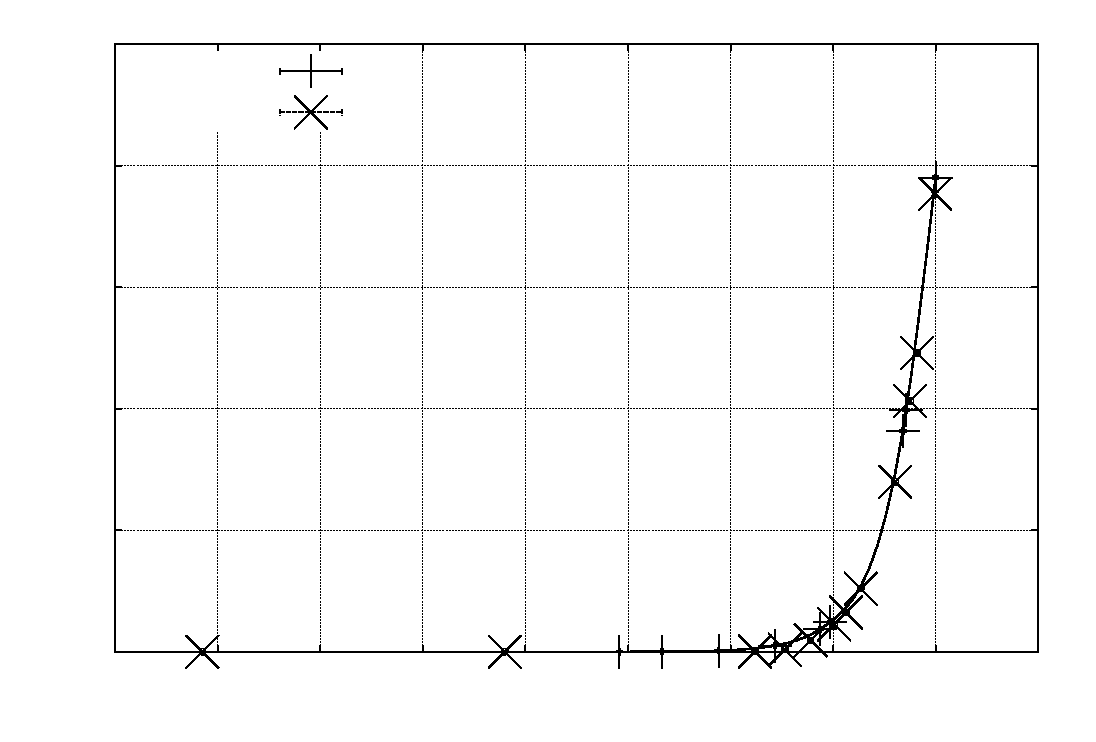
\includegraphics{vstup}}%
    \gplfronttext
  \end{picture}%
\endgroup

\caption{Vstupní charakteristika}
\label{g:vstup}
\end{graph}

Výstupní charakteristiku jsme měřili pro proudy bází $I_B= \SI{0.1}{\milli\ampere}$, \SI{0.2}{\milli\ampere} a \SI{0.3}{\milli\ampere}.
Odpor $R$ jsme nastavili na \SI{20000}{\ohm}.
Naměřené hodnoty jsou uvedeny v tabulce \ref{t:vystup} a zaneseny do grafu \ref{g:vystup}.

\begin{tabulka}[htbp]
\centering
\begin{tabular}{cc||cc||cc}
\multicolumn{2}{c||}{$I_B=\SI{0.1}{\milli\ampere}$} & \multicolumn{2}{c||}{$I_B=\SI{0.2}{\milli\ampere}$} & \multicolumn{2}{c}{$I_B=\SI{0.3}{\milli\ampere}$}
\\ 

$U_{CE}$ (\si{\volt}) & $I_C$ (\si{\milli\ampere}) & $U_{CE}$ (\si{\volt}) & $I_C$ (\si{\milli\ampere}) & $U_{CE}$ (\si{\volt}) & $I_C$ (\si{\milli\ampere}) \\
\hline


\num{0.0066(1)}		& \num{0.048(3)}			& \num{0.0060(1)}		& \num{0.104(3)}			& \num{0.0091(1)}		& \num{0.465(3)} \\
\num{0.0298(1)}		& \num{0.851(3)}			& \num{0.0327(1)}		& \num{2.208(4)}			& \num{0.0218(1)}		& \num{1.891(4)} \\
\num{0.0499(1)}		& \num{2.086(4)}			& \num{0.0716(1)}		& \num{8.466(8)}			& \num{0.0374(1)}		& \num{4.350(5)} \\
\num{0.0815(1)}		& \num{5.089(6)}			& \num{0.1080(1)}		& \num{15.78(2)}			& \num{0.0573(1)}		& \num{8.772(8)} \\
\num{0.1019(1)}		& \num{7.650(7)}			& \num{0.1317(1)}		& \num{19.60(2)}			& \num{0.0832(1)}		& \num{15.92(2)} \\
\num{0.1503(1)}		& \num{10.86(2)}			& \num{0.1624(1)}		& \num{22.73(2)}			& \num{0.1031(1)}		& \num{21.50(2)} \\
\num{0.1733(1)}		& \num{11.60(2)}			& \num{0.2043(1)}		& \num{24.55(2)}			& \num{0.1325(1)}		& \num{28.32(3)} \\
\num{1.005(1)}		& \num{12.30(2)}			& \num{0.3611(1)}		& \num{25.45(3)}			& \num{0.1600(1)}		& \num{32.43(3)} \\
\num{1.505(1)}		& \num{12.32(2)}			& \num{1.061(1)}		& \num{25.58(3)}			& \num{0.8068(1)}		& \num{38.16(3)} \\
\num{2.016(1)}		& \num{12.35(2)}			& \num{2.306(1)}		& \num{25.74(3)}			& \num{1.095(1)}		& \num{38.25(3)} \\
\num{7.565(1)}		& \num{12.54(2)}			& \num{8.765(1)}		& \num{26.34(3)}			& \num{8.203(1)}		& \num{39.54(3)} \\
\num{9.944(1)}		& \num{12.62(2)} & & & & \\										


\end{tabular}
\caption{Výstupní charakteristika}
\label{t:vystup}
\end{tabulka}

\begin{graph}[htbp] 
\centering
% GNUPLOT: LaTeX picture with Postscript
\begingroup
  \makeatletter
  \providecommand\color[2][]{%
    \GenericError{(gnuplot) \space\space\space\@spaces}{%
      Package color not loaded in conjunction with
      terminal option `colourtext'%
    }{See the gnuplot documentation for explanation.%
    }{Either use 'blacktext' in gnuplot or load the package
      color.sty in LaTeX.}%
    \renewcommand\color[2][]{}%
  }%
  \providecommand\includegraphics[2][]{%
    \GenericError{(gnuplot) \space\space\space\@spaces}{%
      Package graphicx or graphics not loaded%
    }{See the gnuplot documentation for explanation.%
    }{The gnuplot epslatex terminal needs graphicx.sty or graphics.sty.}%
    \renewcommand\includegraphics[2][]{}%
  }%
  \providecommand\rotatebox[2]{#2}%
  \@ifundefined{ifGPcolor}{%
    \newif\ifGPcolor
    \GPcolorfalse
  }{}%
  \@ifundefined{ifGPblacktext}{%
    \newif\ifGPblacktext
    \GPblacktexttrue
  }{}%
  % define a \g@addto@macro without @ in the name:
  \let\gplgaddtomacro\g@addto@macro
  % define empty templates for all commands taking text:
  \gdef\gplbacktext{}%
  \gdef\gplfronttext{}%
  \makeatother
  \ifGPblacktext
    % no textcolor at all
    \def\colorrgb#1{}%
    \def\colorgray#1{}%
  \else
    % gray or color?
    \ifGPcolor
      \def\colorrgb#1{\color[rgb]{#1}}%
      \def\colorgray#1{\color[gray]{#1}}%
      \expandafter\def\csname LTw\endcsname{\color{white}}%
      \expandafter\def\csname LTb\endcsname{\color{black}}%
      \expandafter\def\csname LTa\endcsname{\color{black}}%
      \expandafter\def\csname LT0\endcsname{\color[rgb]{1,0,0}}%
      \expandafter\def\csname LT1\endcsname{\color[rgb]{0,1,0}}%
      \expandafter\def\csname LT2\endcsname{\color[rgb]{0,0,1}}%
      \expandafter\def\csname LT3\endcsname{\color[rgb]{1,0,1}}%
      \expandafter\def\csname LT4\endcsname{\color[rgb]{0,1,1}}%
      \expandafter\def\csname LT5\endcsname{\color[rgb]{1,1,0}}%
      \expandafter\def\csname LT6\endcsname{\color[rgb]{0,0,0}}%
      \expandafter\def\csname LT7\endcsname{\color[rgb]{1,0.3,0}}%
      \expandafter\def\csname LT8\endcsname{\color[rgb]{0.5,0.5,0.5}}%
    \else
      % gray
      \def\colorrgb#1{\color{black}}%
      \def\colorgray#1{\color[gray]{#1}}%
      \expandafter\def\csname LTw\endcsname{\color{white}}%
      \expandafter\def\csname LTb\endcsname{\color{black}}%
      \expandafter\def\csname LTa\endcsname{\color{black}}%
      \expandafter\def\csname LT0\endcsname{\color{black}}%
      \expandafter\def\csname LT1\endcsname{\color{black}}%
      \expandafter\def\csname LT2\endcsname{\color{black}}%
      \expandafter\def\csname LT3\endcsname{\color{black}}%
      \expandafter\def\csname LT4\endcsname{\color{black}}%
      \expandafter\def\csname LT5\endcsname{\color{black}}%
      \expandafter\def\csname LT6\endcsname{\color{black}}%
      \expandafter\def\csname LT7\endcsname{\color{black}}%
      \expandafter\def\csname LT8\endcsname{\color{black}}%
    \fi
  \fi
  \setlength{\unitlength}{0.0500bp}%
  \begin{picture}(10204.00,6802.00)%
    \gplgaddtomacro\gplbacktext{%
      \csname LTb\endcsname%
      \put(814,704){\makebox(0,0)[r]{\strut{} 0}}%
      \csname LTb\endcsname%
      \put(814,1871){\makebox(0,0)[r]{\strut{} 10}}%
      \csname LTb\endcsname%
      \put(814,3037){\makebox(0,0)[r]{\strut{} 20}}%
      \csname LTb\endcsname%
      \put(814,4204){\makebox(0,0)[r]{\strut{} 30}}%
      \csname LTb\endcsname%
      \put(814,5370){\makebox(0,0)[r]{\strut{} 40}}%
      \csname LTb\endcsname%
      \put(814,6537){\makebox(0,0)[r]{\strut{} 50}}%
      \csname LTb\endcsname%
      \put(946,484){\makebox(0,0){\strut{} 0}}%
      \csname LTb\endcsname%
      \put(1988,484){\makebox(0,0){\strut{} 0.2}}%
      \csname LTb\endcsname%
      \put(3031,484){\makebox(0,0){\strut{} 0.4}}%
      \csname LTb\endcsname%
      \put(4073,484){\makebox(0,0){\strut{} 0.6}}%
      \csname LTb\endcsname%
      \put(5116,484){\makebox(0,0){\strut{} 0.8}}%
      \csname LTb\endcsname%
      \put(6158,484){\makebox(0,0){\strut{} 1}}%
      \csname LTb\endcsname%
      \put(7201,484){\makebox(0,0){\strut{} 1.2}}%
      \csname LTb\endcsname%
      \put(8243,484){\makebox(0,0){\strut{} 1.4}}%
      \csname LTb\endcsname%
      \put(9286,484){\makebox(0,0){\strut{} 1.6}}%
      \put(176,3620){\rotatebox{-270}{\makebox(0,0){\strut{}$I_B$ (\si{\milli\ampere})}}}%
      \put(5376,154){\makebox(0,0){\strut{}$U_{BE}$ (\si{\volt})}}%
      \csname LT0\endcsname%
      \put(6158,1637){\makebox(0,0)[l]{\strut{}$I_B = \SI{0.1}{\milli\ampere}$}}%
      \csname LT1\endcsname%
      \put(6158,3154){\makebox(0,0)[l]{\strut{}$I_B = \SI{0.2}{\milli\ampere}$}}%
      \csname LT2\endcsname%
      \put(6158,4670){\makebox(0,0)[l]{\strut{}$I_B = \SI{0.3}{\milli\ampere}$}}%
    }%
    \gplgaddtomacro\gplfronttext{%
    }%
    \gplbacktext
    \put(0,0){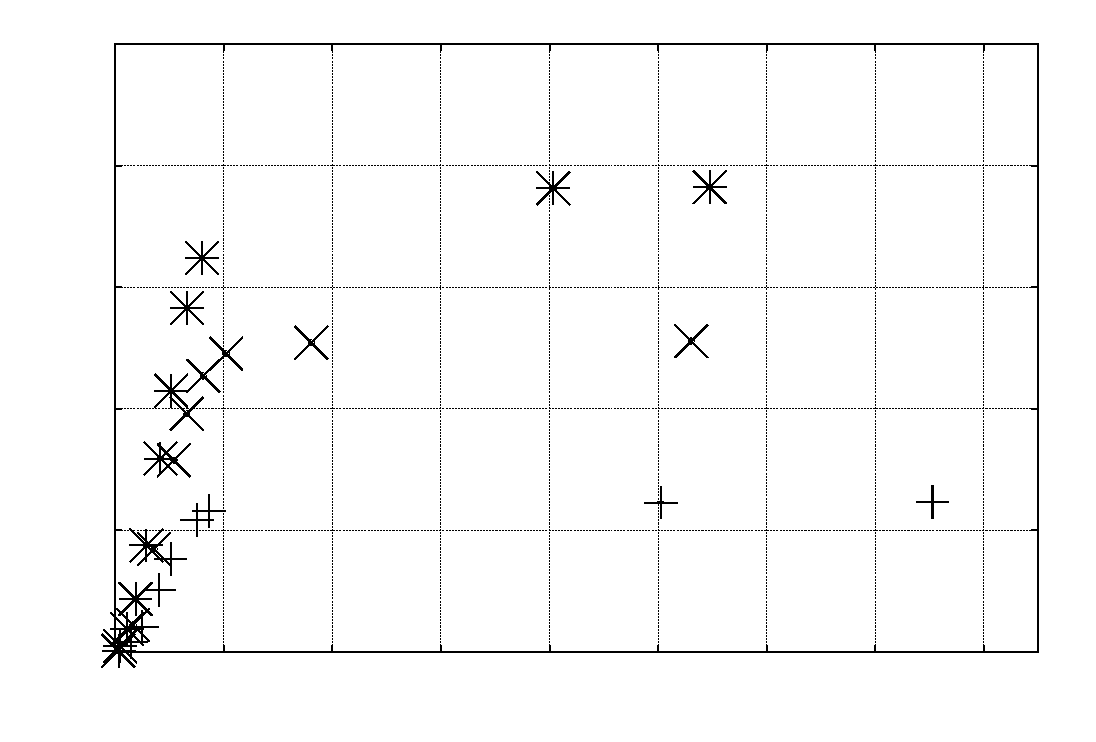
\includegraphics{vystup}}%
    \gplfronttext
  \end{picture}%
\endgroup

\caption{Výstupní charakteristika, některé body ($U_{BE} > \SI{1.6}{\volt}$), byly vynechány, proud je pro vyšší napětí už téměř konstantní}
\label{g:vystup}
\end{graph}

Dále jsme měřili závislost kolektorového proudu na poudu bází pro kolektorová napětí $U_{CE} = \SI{2}{\volt}$, \SI{6}{\volt} a \SI{10}{\volt}.
Naměřené hodnoty jsou uvedeny v tabulce \ref{t:zesil} a zaneseny do grafu \ref{g:zesil}.

\begin{tabulka}[htbp]
\centering
\begin{tabular}{cc||cc||cc}
\multicolumn{2}{c||}{$U_{CE}=\SI{2}{\volt}$} & \multicolumn{2}{c||}{$U_{CE}=\SI{6}{\volt}$} & \multicolumn{2}{c}{$U_{CE}=\SI{10}{\volt}$}
\\ 

$I_B$ (\si{\milli\ampere}) & $I_C$ (\si{\milli\ampere}) & $I_B$ (\si{\milli\ampere}) & $I_C$ (\si{\milli\ampere}) & $I_B$ (\si{\milli\ampere}) & $I_C$ (\si{\milli\ampere}) \\
\hline



\num{0.053(1)}		& \num{6.938(7)}			& \num{0.051(1)}		& \num{6.692(7)}			& \num{0.059(1)}		& \num{7.842(7)} \\
\num{0.082(1)}		& \num{10.698(9)}			& \num{0.092(1)}		& \num{12.17(4)}			& \num{0.101(1)}		& \num{13.52(4)} \\
\num{0.112(1)}		& \num{14.70(4)}			& \num{0.131(1)}		& \num{17.43(4)}			& \num{0.149(1)}		& \num{20.07(4)} \\
\num{0.150(1)}		& \num{19.67(4)}			& \num{0.172(1)}		& \num{22.80(4)}			& \num{0.200(1)}		& \num{27.02(4)} \\
\num{0.194(1)}		& \num{25.37(4)}			& \num{0.200(1)}		& \num{26.59(5)}			& \num{0.250(2)}		& \num{33.82(5)} \\
\num{0.228(1)}		& \num{29.68(5)}			& \num{0.232(1)}		& \num{30.78(5)}			& \num{0.299(2)}		& \num{40.56(5)} \\
\num{0.251(2)}		& \num{32.68(5)}			& \num{0.259(2)}		& \num{34.46(5)}					& & \\
\num{0.295(2)}		& \num{38.39(5)}			& \num{0.298(2)}		& \num{39.62(5)}					& & \\

\end{tabular}
\caption{Závislost kolektorového proudu na bázovém proudu}
\label{t:zesil}
\end{tabulka}

\begin{graph}[htbp] 
\centering
% GNUPLOT: LaTeX picture with Postscript
\begingroup
  \makeatletter
  \providecommand\color[2][]{%
    \GenericError{(gnuplot) \space\space\space\@spaces}{%
      Package color not loaded in conjunction with
      terminal option `colourtext'%
    }{See the gnuplot documentation for explanation.%
    }{Either use 'blacktext' in gnuplot or load the package
      color.sty in LaTeX.}%
    \renewcommand\color[2][]{}%
  }%
  \providecommand\includegraphics[2][]{%
    \GenericError{(gnuplot) \space\space\space\@spaces}{%
      Package graphicx or graphics not loaded%
    }{See the gnuplot documentation for explanation.%
    }{The gnuplot epslatex terminal needs graphicx.sty or graphics.sty.}%
    \renewcommand\includegraphics[2][]{}%
  }%
  \providecommand\rotatebox[2]{#2}%
  \@ifundefined{ifGPcolor}{%
    \newif\ifGPcolor
    \GPcolorfalse
  }{}%
  \@ifundefined{ifGPblacktext}{%
    \newif\ifGPblacktext
    \GPblacktexttrue
  }{}%
  % define a \g@addto@macro without @ in the name:
  \let\gplgaddtomacro\g@addto@macro
  % define empty templates for all commands taking text:
  \gdef\gplbacktext{}%
  \gdef\gplfronttext{}%
  \makeatother
  \ifGPblacktext
    % no textcolor at all
    \def\colorrgb#1{}%
    \def\colorgray#1{}%
  \else
    % gray or color?
    \ifGPcolor
      \def\colorrgb#1{\color[rgb]{#1}}%
      \def\colorgray#1{\color[gray]{#1}}%
      \expandafter\def\csname LTw\endcsname{\color{white}}%
      \expandafter\def\csname LTb\endcsname{\color{black}}%
      \expandafter\def\csname LTa\endcsname{\color{black}}%
      \expandafter\def\csname LT0\endcsname{\color[rgb]{1,0,0}}%
      \expandafter\def\csname LT1\endcsname{\color[rgb]{0,1,0}}%
      \expandafter\def\csname LT2\endcsname{\color[rgb]{0,0,1}}%
      \expandafter\def\csname LT3\endcsname{\color[rgb]{1,0,1}}%
      \expandafter\def\csname LT4\endcsname{\color[rgb]{0,1,1}}%
      \expandafter\def\csname LT5\endcsname{\color[rgb]{1,1,0}}%
      \expandafter\def\csname LT6\endcsname{\color[rgb]{0,0,0}}%
      \expandafter\def\csname LT7\endcsname{\color[rgb]{1,0.3,0}}%
      \expandafter\def\csname LT8\endcsname{\color[rgb]{0.5,0.5,0.5}}%
    \else
      % gray
      \def\colorrgb#1{\color{black}}%
      \def\colorgray#1{\color[gray]{#1}}%
      \expandafter\def\csname LTw\endcsname{\color{white}}%
      \expandafter\def\csname LTb\endcsname{\color{black}}%
      \expandafter\def\csname LTa\endcsname{\color{black}}%
      \expandafter\def\csname LT0\endcsname{\color{black}}%
      \expandafter\def\csname LT1\endcsname{\color{black}}%
      \expandafter\def\csname LT2\endcsname{\color{black}}%
      \expandafter\def\csname LT3\endcsname{\color{black}}%
      \expandafter\def\csname LT4\endcsname{\color{black}}%
      \expandafter\def\csname LT5\endcsname{\color{black}}%
      \expandafter\def\csname LT6\endcsname{\color{black}}%
      \expandafter\def\csname LT7\endcsname{\color{black}}%
      \expandafter\def\csname LT8\endcsname{\color{black}}%
    \fi
  \fi
  \setlength{\unitlength}{0.0500bp}%
  \begin{picture}(10204.00,6802.00)%
    \gplgaddtomacro\gplbacktext{%
      \csname LTb\endcsname%
      \put(814,704){\makebox(0,0)[r]{\strut{} 0}}%
      \csname LTb\endcsname%
      \put(814,1871){\makebox(0,0)[r]{\strut{} 10}}%
      \csname LTb\endcsname%
      \put(814,3037){\makebox(0,0)[r]{\strut{} 20}}%
      \csname LTb\endcsname%
      \put(814,4204){\makebox(0,0)[r]{\strut{} 30}}%
      \csname LTb\endcsname%
      \put(814,5370){\makebox(0,0)[r]{\strut{} 40}}%
      \csname LTb\endcsname%
      \put(814,6537){\makebox(0,0)[r]{\strut{} 50}}%
      \csname LTb\endcsname%
      \put(946,484){\makebox(0,0){\strut{} 0}}%
      \csname LTb\endcsname%
      \put(2212,484){\makebox(0,0){\strut{} 0.05}}%
      \csname LTb\endcsname%
      \put(3478,484){\makebox(0,0){\strut{} 0.1}}%
      \csname LTb\endcsname%
      \put(4744,484){\makebox(0,0){\strut{} 0.15}}%
      \csname LTb\endcsname%
      \put(6009,484){\makebox(0,0){\strut{} 0.2}}%
      \csname LTb\endcsname%
      \put(7275,484){\makebox(0,0){\strut{} 0.25}}%
      \csname LTb\endcsname%
      \put(8541,484){\makebox(0,0){\strut{} 0.3}}%
      \csname LTb\endcsname%
      \put(9807,484){\makebox(0,0){\strut{} 0.35}}%
      \put(176,3620){\rotatebox{-270}{\makebox(0,0){\strut{}$I_C$ (\si{\milli\ampere})}}}%
      \put(5376,154){\makebox(0,0){\strut{}$I_B$ (\si{\milli\ampere})}}%
    }%
    \gplgaddtomacro\gplfronttext{%
      \csname LTb\endcsname%
      \put(2134,6278){\makebox(0,0)[r]{\strut{}$U_{BE}=\SI{2}{\volt}$}}%
      \csname LTb\endcsname%
      \put(2134,5885){\makebox(0,0)[r]{\strut{}$U_{BE}=\SI{6}{\volt}$}}%
      \csname LTb\endcsname%
      \put(2134,5492){\makebox(0,0)[r]{\strut{}$U_{BE}=\SI{10}{\volt}$}}%
    }%
    \gplbacktext
    \put(0,0){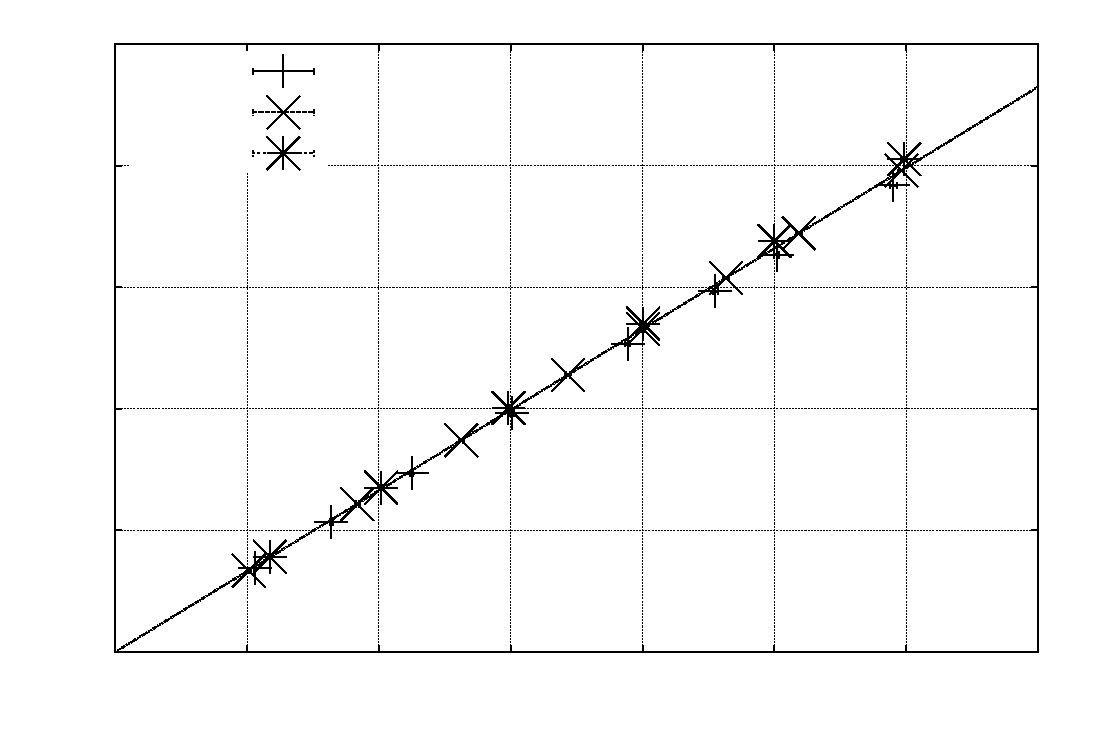
\includegraphics{zesil}}%
    \gplfronttext
  \end{picture}%
\endgroup

\caption{Závislost kolektorového proudu na bázovém proudu}
\label{g:zesil}
\end{graph}

Pomocí linární regrese závislosti $I_{CE}=f(I{BE})$ jsme určili činitel proudového zesílení $\beta = \num[separate-uncertainty=true]{133(2)}$.